%!TEX root = ../../main.tex

<<<<<<< HEAD
\chapter{Ansprechpartner und Organisationsstruktur}
Die Zuständigkeiten und die allgemeine personelle Organisationsstruktur sind dem Organigramm in Abbildung \ref{fib:Organigramm} zu entnehmen.
\begin{figure}[h]
\centering
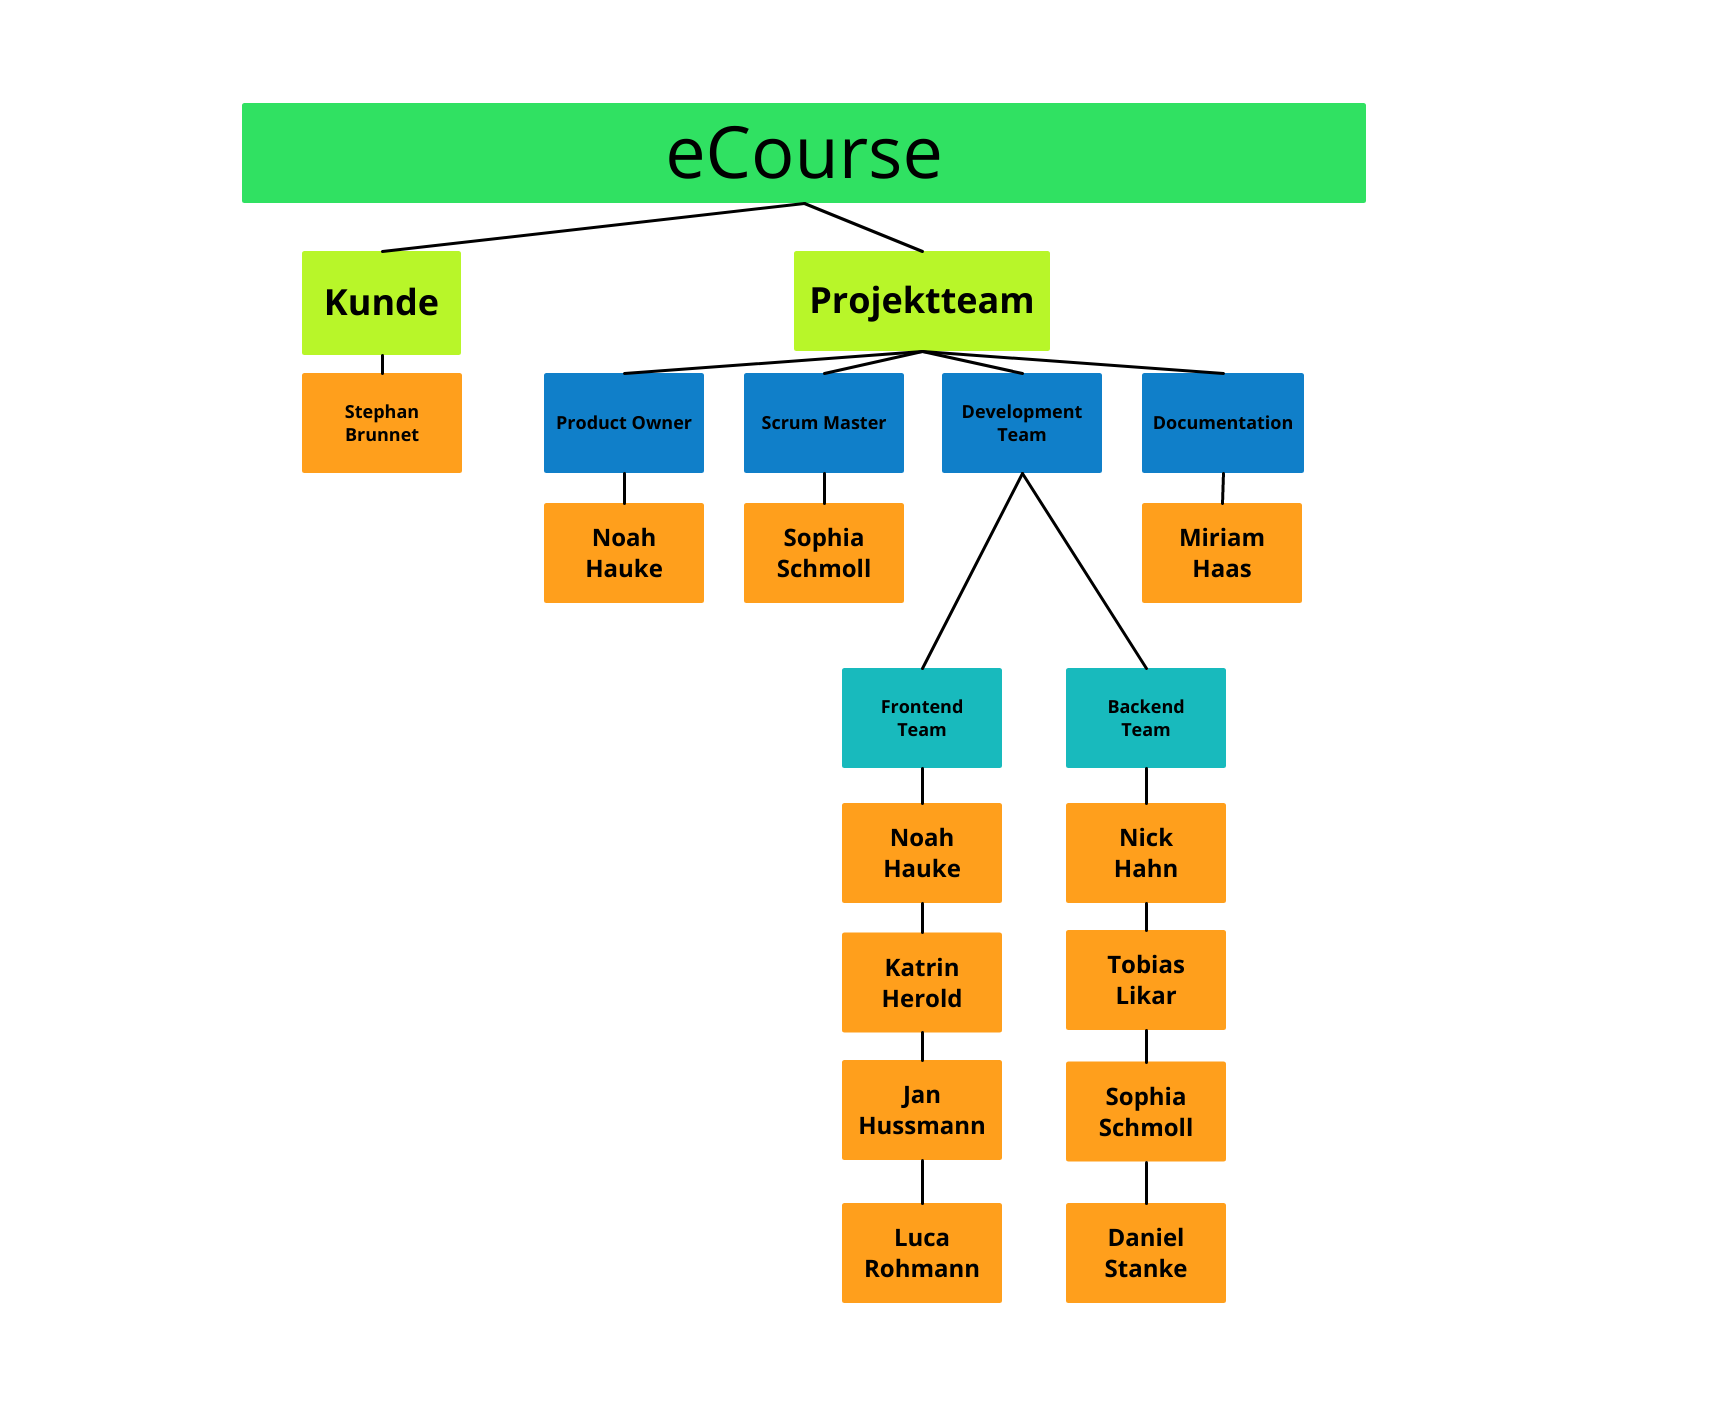
\includegraphics[height=.8\textwidth]{Organigramm.png}
\caption{Organigramm für das Projekt eCourse}
\label{fib:Organigramm}
\end{figure}\\

Alle externe Anfragen an das Projektteam gehen über den Projektansprechpartner. Diese Rolle übernimmt Miriam Haas. Als Kontaktart wird eine E-Mail an \href{mailto:inf19109@lehre.dhbw-stuttgart.de}{diese Adresse} bevorzugt. 
=======
\chapter{Projekthandbuch}
%!TEX root = ../../main.tex

\chapter{Ansprechpartner}
Die Zuständigkeiten und die allgemeine personelle Organisationsstruktur sind dem Organigramm in Abbildung \textcolor{magenta}{Hier das Organigramm referenzieren} zu entnehmen.
Die, für dieses Projekt, verantwortlichen Personen sind der Tabelle \ref{tab:Ansprechpartner} zu entnehmen.

\begin{table} [H]
\centering
\begin{tabular} {|c|c|} 
\hline
Rolle im Projekt & Name \\
\hline
Stakeholder & Stephan Brunnet  \\
\hline
Scrum-Master und Development-Team & Noah Hauke \\
\hline
Product-Owner und Development-Team & Sophia Schmoll \\
\hline
Development-Team & Miriam Haas \\
\hline
Development-Team & Nick Hahn \\
\hline
Development-Team & Katrin Herold \\
\hline
Development-Team & Jan Hussmann \\
\hline
Development-Team & Tobias Likar \\
\hline
Development-Team & Luca Rohmann \\
\hline
Development-Team & Daniel Stanke \\
\hline
\end{tabular}
\caption{verfügbare Datentypen in der Programmierung der PSS 4000}
\label{tab:Ansprechpartner}
\end{table}
>>>>>>> Documentation_Pflichtenheft
